\section{Sorting}
\label{sec:sorting}

One of the most fundamental operations in computer science is sorting a sequence of elements. And as old as the problem is as numerous are the algorithms to solve it. These sorting algorithms differ in various aspects such as best, average and worst runtime or memory complexity, stability, the number of comparisons and swaps and whether the algorithm is a comparison sort or not.

The sort implementations provided by todays standard libraries are highly tuned achieving an optimal asymptotic runtime complexity which is $\mathcal{O}(n log n)$ for comparison based sorts. Examples would be variations of quick sort (C), merge sort (C++), intro sort (C++, .NET) or Timsort (Java, Python). All these algorithms are comparison sorts, thus requiring a method of comparing two elements of the input sequence. This comparison is often provided either by the language or standard library (e.g. $<$ operator) or by the programmer via a custom comparison function giving the flexibility to compare and sort any kind of elements.

Another class of sorting methods are integer sorting algorithms. These algorithms do not use comparisons to determine the order of elements but rely on more flexible integer arithmetic applied to the keys which should be sorted. Therefore, they can achieve a better asymptotic runtime complexity than comparison based ones. Popular algorithms of this kind are radix sort, counting sort and bucket sort. All of them running with $\mathcal{O}(n + k)$ or $\mathcal{O}(n * k)$ (where k is a constant) in linear time.
However, despite their key limitation, integer sorting algorithms also work on other kind of types as long as they can be represented as integers in binary (e.g. strings can be seen as byte array forming a (larger) integer).

Considering parallelizability and an eventual GPU implementation, sorting lies between matrix multiplication and prefix sum offering some degree of parallelism depending on the chosen algorithm. The following chapter will focus on the implementation of two widely chosen algorithms for GPU sorting. These are the comparison based bitonic sorting network and the integer sorting algorithm radix sort. To reduce complexity (especially of the latter), the input arrays consist of unsigned integers.


\subsection{CPU Implementation}


quicksort, radix sort

\subsection{GPU Implementations}

\subsubsection{Bitonic Sort}
parallelism on the cost of complexity

Ken Batcher

\begin{figure}
\centering
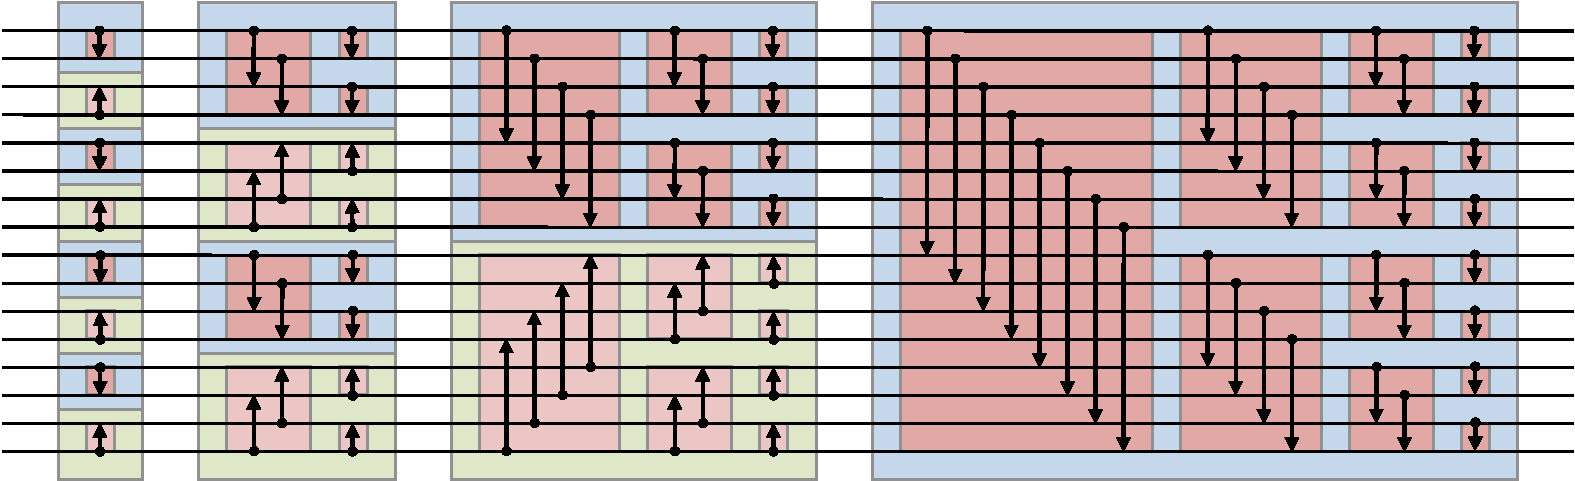
\includegraphics[width=0.8\linewidth]{bitonic_sort}
\caption{Example of a bitonic sorting network for 16 inputs \cite{wiki_bitonic_sort}.}
\label{fig:bitonic_sort}
\end{figure}

approach
kernel code/host code with explanation
improvements
runtime (diagram), $n * n \log^2(n)$, why still faster than CPU?

\subsubsection{Radix Sort}
\label{sec:sorting_radix}
integer only
seems easy to parallelize, problems? (order of work item execution)

kernel code/ host code (AMD/NVIDIA)

runtime (diagram)

\subsection{Existing implementations}
libCL
AMD APP SDK Samples
NVIDIA OpenCL Samples
clpp
